\chapter{Automate du texte}
\label{chap-text-automaton}
\index{Automate!du texte}
Les langues naturelles contiennent beaucoup d’ambiguïtés lexicales. L’automate du texte
est un moyen efficace et visuel de représenter ces ambiguïtés. Chaque phrase du texte est
représentée par un automate dont les chemins expriment toutes les interprétations possibles.


\bigskip
\noindent Ce chapitre présente les automates de texte, le détail de leur construction ainsi
que les opérations qui peuvent leur être appliquées, en particulier la levée d’ambiguïtés au moyen
du programme ELAG. Depuis la version 2.1, il est possible d’effectuer des recherches de
motifs sur l’automate du texte (voir section \ref{section-locate-tfst}).


\section{Présentation} \index{Dictionnaire!du texte}
L’automate du texte permet d’exprimer toutes les interprétations lexicales possibles des
mots. Ces différentes interprétations sont les différentes entrées présentes dans les
dictionnaires du texte. La figure~\ref{fig-sentence-automaton} montre l’automate de la
quatrième phrase du texte \textit{Ivanhoe}.

\begin{figure}[!ht]
\begin{center}
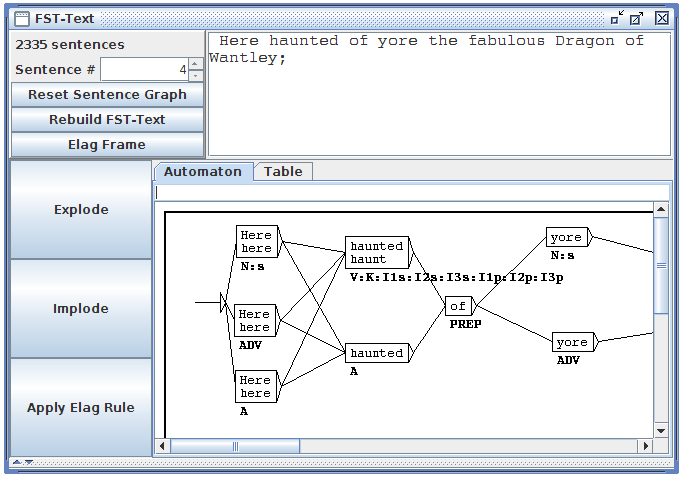
\includegraphics[width=15.5cm]{resources/img/fig7-1.png}
\caption{Exemple d’automate de phrase\label{fig-sentence-automaton}}
\end{center}
\end{figure}

\bigskip
\noindent On peut voir sur la figure~\ref{fig-sentence-automaton}
que le mot \verb+Here+ possède ici trois interprétations (adjectif, adverbe et nom),
\verb+haunted+ deux (adjectif et verbe), etc. Toutes les combinaisons possibles
sont exprimées, car chaque interprétation de chaque mot est reliée à toutes les interprétations
des mots suivants et précédents.


\bigskip
\noindent En cas de concurrence entre un mot composé et une séquence de mots simples, 
l’automate contient un chemin étiqueté par le mot composé, parallèle aux chemins exprimant
les combinaisons de mots simples. Ceci est illustré par la figure~\ref{fig-overlap}, 
où le mot composé \texttt{courts of law} est concurrent avec une combinaison de mots simples.

\begin{figure}[!ht]
\begin{center}
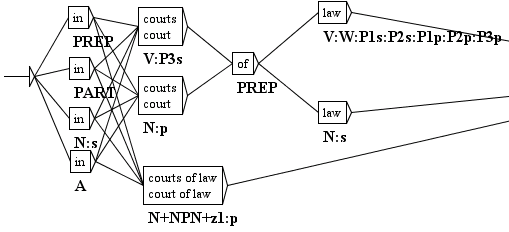
\includegraphics[width=12.5cm]{resources/img/fig7-2.png}
\caption{Concurrence entre un mot composé et une combinaison de mots simples\label{fig-overlap}}
\end{center}
\end{figure}

\bigskip
\noindent Par construction, l’automate du texte ne contient pas de boucle. On dit que l’automate
du texte est \textit{acyclique}.\index{Automate!acyclique}

\bigskip
\noindent NOTE: le terme ``automate du texte'' est un abus de langage. En effet, il y a en
réalité un automate pour chaque phrase du texte. Cependant, la concaténation de tous ces automates
correspondrait à l’automate de tout le texte. On utilise donc le terme ``automate du texte'' 
même si l’on ne manipule pas réellement cet objet pour des raisons pratiques.

\section{Construction}
\label{construction-text-automaton}
Pour construire l’automate d’un texte, vous devez ouvrir ce texte, puis cliquer dans le menu "Text"
sur "Construct FST-Text...". Il est recommandé d’avoir découpé le texte en phrases et
de lui avoir appliqué les dictionnaires. Si vous n’avez pas découpé le texte en phrases, le
programme de construction découpera arbitrairement le texte en séquences de 2000 unités
lexicales au lieu de construire un automate par phrase. Si vous n’avez pas appliqué les 
dictionnaires, les automates de phrase que vous obtiendrez ne seront constitués que d’un seul
chemin ne comportant que des mots inconnus.



\subsection{Règles de construction de l’automate du texte}
\index{Granularité des dictionnaires}\index{Dictionnaire!granularité}\index{Degré d'ambiguïté}
Les automates de phrase sont construits à partir des dictionnaires du texte. Le degré
d’ambiguïté obtenu est donc directement lié à la finesse de description des dictionnaires utilisés.
Sur l’automate de phrase de la figure~\ref{fig-ambiguity-of-which}, on peut voir que le mot
\verb+which+ a été codé deux fois comme déterminant dans deux sous-catégories de la catégorie
 \verb+DET+. Cette finesse de description ne sera d’aucune utilité si l’on ne s’intéresse qu’à la
 catégorie grammaticale de ce mot. Il faut donc adapter la finesse des dictionnaires à l’utilisation
 recherchée.


\begin{figure}[!ht]
\begin{center}
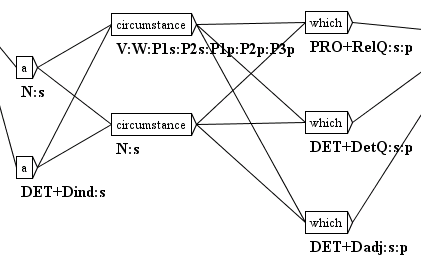
\includegraphics[width=10.6cm]{resources/img/fig7-3.png}
\caption{Double entrée pour \texttt{which} en tant que déterminant\label{fig-ambiguity-of-which}}
\end{center}
\end{figure}

\bigskip
\noindent Pour chaque unité lexicale de la phrase, Unitex recherche toutes ses interprétations
possibles dans le dictionnaire des mots simples du texte. On recherche ensuite toutes les suites
d’unités lexicales qui ont une interprétation dans le dictionnaire des mots composés du
texte. Toutes les combinaisons de ces interprétations forment l’automate de la phrase.


\bigskip
\noindent NOTE : quand le texte contient des étiquettes lexicales (\textit{e.g.}
 \verb${aujourd’hui,.ADV}$), ces étiquettes sont reproduites à l’identique dans l’automate, 
sans que le programme essaye de décomposer les séquences qu’elles représentent.\index{Étiquette lexicale}

\bigskip
\noindent Dans chaque boîte, la $1\iere$  ligne contient la forme fléchie trouvée dans le texte, et
la $2\ieme$ ligne contient la forme canonique si elle est différente. Les autres informations sont
codées sous la boîte (voir section~\ref{section-displaying-sentence-automata}).

\bigskip
\noindent Les espaces séparant les unités lexicales ne sont pas retranscrits dans l’automate, 
à l’exception des espaces à l’intérieur de mots composés.


\bigskip
\noindent La casse des unités lexicales est conservée. Par exemple, si l’on trouve le mot
\verb+Here+, on conserve la majuscule (voir figure~\ref{fig-sentence-automaton}). Ce choix permet 
de ne pas perdre cette information lors du passage à l’automate du texte, ce qui pourra être utile
pour des applications où la casse est importante, telle que la reconnaissance des noms propres.


\subsection{Normalisation de formes ambiguës}
\index{Normalisation!de l'automate du texte}\index{Normalisation!de formes ambiguës}
\index{Texte!automate du!normalisation}
Lors de la construction de l’automate, il est possible d’effectuer une normalisation de
formes ambiguës en appliquant une grammaire de normalisation. Cette grammaire doit
se nommer \verb+Norm.fst2+ et doit être placée dans votre répertoire personnel, dans le sous-répertoire
 \verb+/Graphs/Normalization+ de la langue voulue. Les grammaires de normalisation de formes ambiguës sont décrites à la section~\ref{section-normalizing-text-automataon}.

\bigskip
\noindent Si une séquence du texte est reconnue par la grammaire de normalisation, toutes les
interprétations décrites par la grammaire sont insérées dans l’automate du texte. La figure
~\ref{fig-example-tfst-normalization-graph} montre l’extrait de la grammaire utilisée pour
le français qui explicite l’ambiguïté de la séquence \verb+l'+.

\begin{figure}[!ht]
\begin{center}
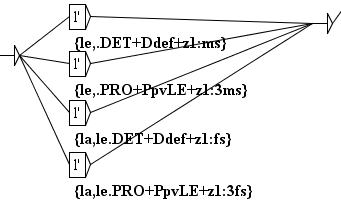
\includegraphics[width=8.6cm]{resources/img/fig7-4.png}
\caption{Normalisation de la séquence \texttt{l'}\label{fig-example-tfst-normalization-graph}}
\end{center}
\end{figure}

\bigskip
\noindent Si l’on applique cette grammaire à une phrase française contenant la séquence
\verb+l'+, on obtient un automate de phrase similaire à celui de la figure ~\ref{fig-tfst-normalization-results}.

\begin{figure}[!ht]
\begin{center}
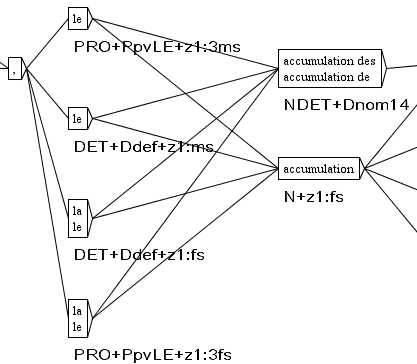
\includegraphics[width=10.2cm]{resources/img/fig7-5.png}
\caption{Automate normalisé avec la grammaire de la figure~\ref{fig-example-tfst-normalization-graph}
\label{fig-tfst-normalization-results}}
\end{center}
\end{figure}

\bigskip
\noindent Dans l’automate obtenu, on peut voir que les quatre règles de réécriture de la séquence
\verb+l'+ ont été appliquées, ce qui a ajouté quatre étiquettes dans l’automate.
%These labels are not concurrent with the two preexisting paths for the sequence \verb+l'+,
%because of the "keep best paths" heuristic (see section \ref{section-keeping-best-paths}).
Ces étiquettes ne sont pas concurrentes avec les deux chemins préexistants pour la séquence
\verb+l’+ grâce à l'heuristique "keep best paths" (voir section \ref{section-keeping-best-paths}).
La normalisation à la construction de l’automate du texte permet d’ajouter des chemins à l’automate,
pas d’en supprimer.
%Removing paths will be partially done by the "keep best paths" heuristic, if enabled. To go
%further,
%you will need to use the ELAG disambiguation functionality.
La suppression des chemins est partiellement faite par l'heuristique "keep best paths" si elle est
sélectionnée. Pour aller plus loin, vous devez utiliser les fonctionnalités de désambïguisation du
système ELAG

\subsection{Normalisation des pronoms clitiques en portugais}
\label{section-portuguese-clitics}
\index{Clitiques!normalisation}\index{Normalisation!des clitiques en portugais}
\index{Portugais!normalisation des clitiques}
En portugais, les verbes au futur et au conditionnel peuvent être modifiés par l’inser-
tion d’un ou deux pronoms clitiques entre le radical et le suffixe du verbe. Par exemple, la
séquence \textit{dir-me-ão} (\textit{ils me diront}), correspond à la forme verbale complète 
\textit{dirão}, associée au pronom \textit{me}. En vue de pouvoir effectuer des manipulations
sur cette forme sous-jacente, il est nécessaire de l’introduire dans l’automate du texte, en parallèle
avec la séquence d’origine. Ainsi, l’utilisateur pourra rechercher l’une ou l’autre forme selon ses besoins. 
Les figures~\ref{fig-1285-not-normalized} et~\ref{fig-1285-normalized} montrent l’automate d’une phrase
avant et après normalisation des clitiques.


\begin{figure}[!ht]
\begin{center}
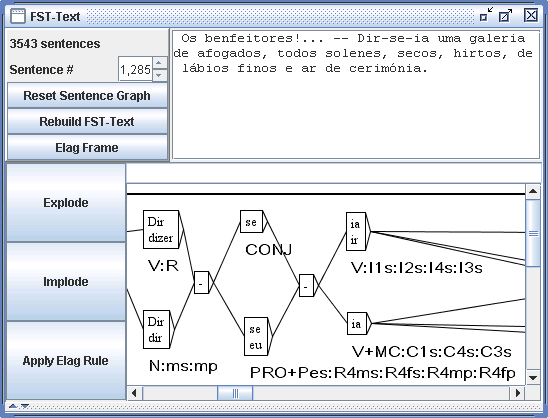
\includegraphics[width=11cm]{resources/img/fig7-6.png}
\caption{Automate de phrase non normalisé\label{fig-1285-not-normalized}}
\end{center}
\end{figure}
\begin{figure}[!ht]
\begin{center}
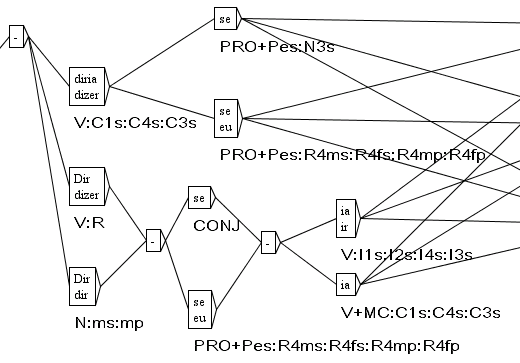
\includegraphics[width=11cm]{resources/img/fig7-7.png}
\caption{Automate de phrase normalisé\label{fig-1285-normalized}}
\end{center}
\end{figure}
\clearpage

\index{Programmes externes!\verbc{Reconstrucao}}\index{\verbc{Reconstrucao}}
\bigskip
\noindent Le programme \verb+Reconstrucao+ permet de construire dynamiquement pour chaque texte
une grammaire de normalisation de ces formes. La grammaire ainsi produite peut alors être
utilisée pour normaliser l’automate du texte. La fenêtre de configuration de construction de
l’automate propose l’option "Build clitic normalization grammar" (voir figure
~\ref{fig-Txt2Tfst-configuration}). Cette option lance automatiquement la construction de la 
grammaire de normalisation, qui est ensuite utilisée pour construire l’automate du texte, 
si vous avez sélectionné l’option "Apply the Normalization grammar".




\subsection{Conservation des meilleurs chemins}
\label{section-keeping-best-paths}
\index{Conservation des meilleurs chemins}
Il peut arriver qu’un mot inconnu vienne parasiter l’automate du texte en étant concurrent avec une
séquence complètement étiquetée. Ainsi, dans l’automate de phrase de la
figure~\ref{fig-unknown-word-ambiguity}, on peut voir que l’adverbe \verb+aujourd'hui+ est
concurrencé par le mot inconnu \verb+aujourd+, suivi d’une apostrophe et du participe passé du verbe
\verb+huir+.


\begin{figure}[!ht]
\begin{center}
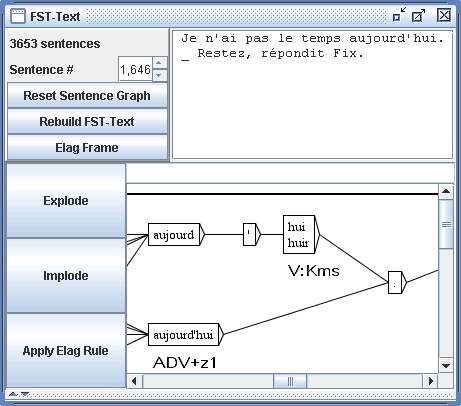
\includegraphics[width=11.6cm]{resources/img/fig7-8.png}
\caption{Ambiguïté due à une séquence contenant un mot inconnu\label{fig-unknown-word-ambiguity}}
\end{center}
\end{figure}

\begin{figure}[!ht]
\begin{center}
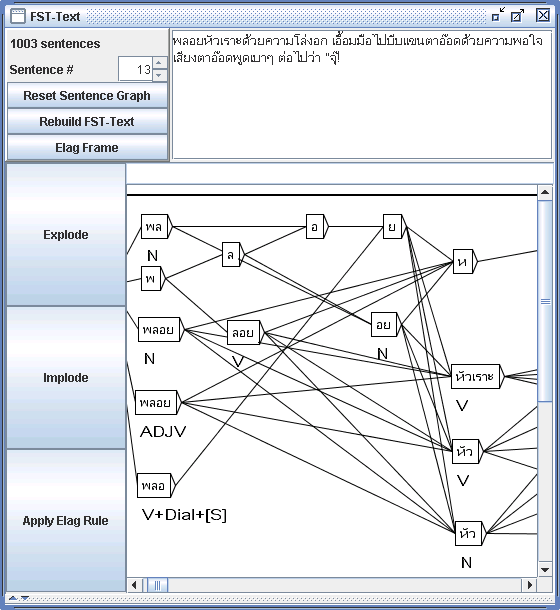
\includegraphics[width=14cm]{resources/img/fig7-9.png}
\caption{Automate d’une phrase thaï\label{fig-thai-sentence-automaton}}
\end{center}
\end{figure}

\bigskip
\noindent On trouve également ce phénomène dans le traitement de certaines langues asiatiques
comme le thaï. Quand les mots ne sont pas délimités, il n’y a pas d’autre solution que d’envisager
toutes les combinaisons possibles, ce qui entraîne la création de nombreux chemins
comportant des mots inconnus qui s’entremêlent avec les chemins étiquetés. La figure
~\ref{fig-thai-sentence-automaton} montre un exemple d’un tel automate de phrase en thaï.

\bigskip
\noindent Il est possible de supprimer ces chemins parasites. Pour cela, il faut sélectionner l’option
"Clean Text FST" dans la fenêtre de configuration de la construction de l’automate du texte
(voir figure~\ref{fig-Txt2Tfst-configuration}). Cette option indique au programme de construction de
l’automate qu’il doit nettoyer chaque automate de phrase.


\begin{figure}[!ht]
\begin{center}
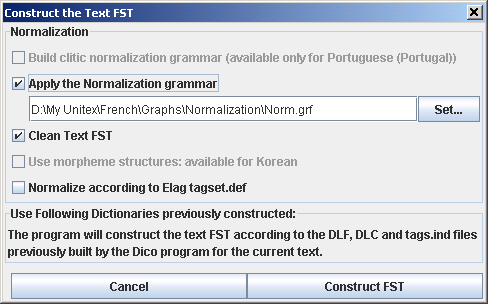
\includegraphics[width=14cm]{resources/img/fig7-10.png}
\caption{Configuration de la construction de l’automate du texte
\label{fig-Txt2Tfst-configuration}}
\end{center}
\end{figure}

\bigskip
\noindent Ce nettoyage s’effectue selon le principe suivant : si plusieurs chemins sont en
concurrence dans l’automate, le programme garde ceux qui contiennent le moins de mots inconnus. Par
exemple, la séquence. \verb+aujourd'hui+ en tant qu’adverbe composé l’emporte sur la décomposition
en \verb+aujourd+ suivi d’une apostrophe et de \verb+hui+, car \verb+aujourd+ est un mot inconnu,
ce qui fait une forme non étiquetée contre zéro dans le cas de l’adverbe composé. La
figure~\ref{fig-clean-thai-sentence-automaton} montre l’automate de la
figure~\ref{fig-thai-sentence-automaton} après nettoyage.

\begin{figure}[!ht]
\begin{center}
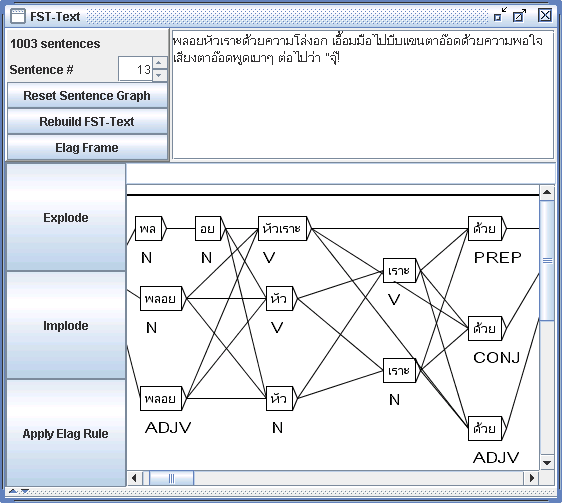
\includegraphics[width=10cm]{resources/img/fig7-11.png}
\caption{Automate de la figure~\ref{fig-thai-sentence-automaton} après nettoyage\label{fig-clean-thai-sentence-automaton}}
\end{center}
\end{figure}

%\clearpage

\section{Levée d’ambiguïtés lexicales avec ELAG}
\index{Levée d’ambiguïtés}\index{ELAG}
Le programme ELAG permet d’appliquer des grammaires de levée d’ambiguïtés sur
l’automate du texte. C’est un mécanisme puissant qui permet à chacun d’écrire ses propres
règles de façon indépendante des règles déjà existantes. Cette section présente rapidement le
formalisme des grammaires utilisées par ELAG ainsi que le fonctionnement du programme.
Pour plus de détails, le lecteur pourra se reporter à \cite{elag-blanc-dister} et \cite{ELAG}.


\subsection{Grammaires de levée d’ambiguïtés}
\label{section-elag-grammars}
\index{Grammaires!levée d’ambiguïtés}
Les grammaires manipulées par ELAG ont une syntaxe particulière. Elles comportent deux parties, que
nous appelerons partie \textit{si} et \textit{alors}. La partie \textit{si} d’une grammaire
ELAG se divise en deux zones délimitées par des boîtes contenant le symbole \verb+<!>+. 
La partie \textit{alors} est divisée de la même façon au moyen du symbole \verb+<=>+.                                                                 La signification d’une grammaire est la suivante : dans l’automate du texte, si l’on trouve une
séquence reconnue par la partie \textit{si} alors elle doit aussi être reconnue par la partie
\textit{alors} de la grammaire, faute de quoi elle sera retirée de l’automate du texte.


\begin{figure}[!ht]
\begin{center}
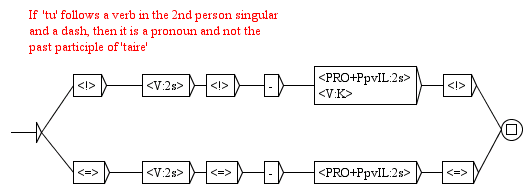
\includegraphics[width=13.1cm]{resources/img/fig7-12.png}
\caption{Exemple de grammaire ELAG \texttt{elag-tu.grf}\label{fig-elag-tu}}
\end{center}
\end{figure}

\bigskip
\noindent La figure~\ref{fig-elag-tu} montre un exemple de grammaire. La partie
\textit{si} reconnait un verbe à la deuxième personne du singulier suivi par un tiret et
\verb+tu+, soit en tant que pronom, soit en tant que participe passé du verbe \verb+taire+. 
La partie \textit{alors} impose que \verb+tu+ soit alors considéré comme pronom. 
La figure~\ref{fig-applying-tu-grammar} montre le résultat de l’application de cette
grammaire sur la phrase "\textit{Feras-tu cela bientôt$~$?}". On peut voir sur l’automate
du bas que le chemin correspondant à \verb+tu+ participe passé a été éliminé.


\begin{figure}[!ht]
\begin{center}
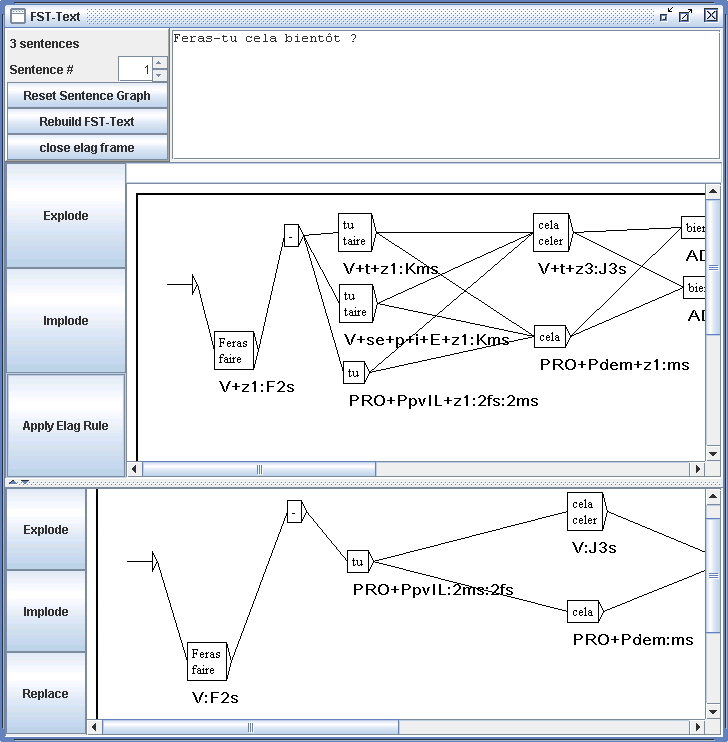
\includegraphics[width=14cm]{resources/img/fig7-13.png}
\caption{Résultat de l’application de la grammaire de la figure~\ref{fig-elag-tu}
\label{fig-applying-tu-grammar}}
\end{center}
\end{figure}

\begin{figure}[!ht]
\begin{center}
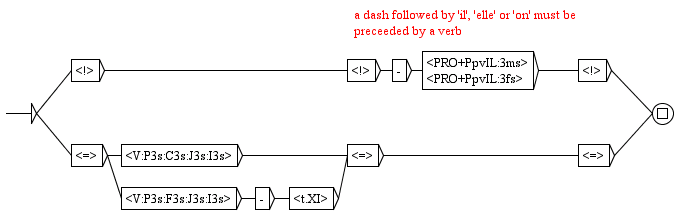
\includegraphics[width=14cm]{resources/img/fig7-14.png}
\caption{Utilisation du point de sychronisation\label{fig-synchronization-point}}
\end{center}
\end{figure}

\subsubsection{Point de synchronisation}
\index{Point de synchronisation}
Les parties \textit{si} et \textit{alors} d’une grammaire ELAG sont divisées en deux par le
deuxième symbole \verb+<!>+ dans la partie  \textit{si}, et par le deuxième symbole \verb+<=>+
dans la partie \textit{alors}.
Ces symboles forment un \textit{point de synchronisation}.
Cela permet d’écrire des règles dans lesquelles les contraintes \textit{si} et \textit{alors} 
ne sont pas nécessairement alignées, comme c’est par exemple le
cas sur la figure~\ref{fig-synchronization-point}. Cette grammaire s’interprète de la manière 
suivante : si on trouve un tiret suivi par \verb+il+, \verb+elle+ ou \verb+on+, alors ce tiret
doit être précédé par un verbe, éventuellement suivi de \verb+-t+. Ainsi, si l’on considère
la phrase de la figure~\ref{fig-est-il} commençant par \textit{Est-il}, on peut voir que toutes
les interprétations non verbales de \verb+Est+ ont été supprimées.


\begin{figure}[!ht]
\begin{center}
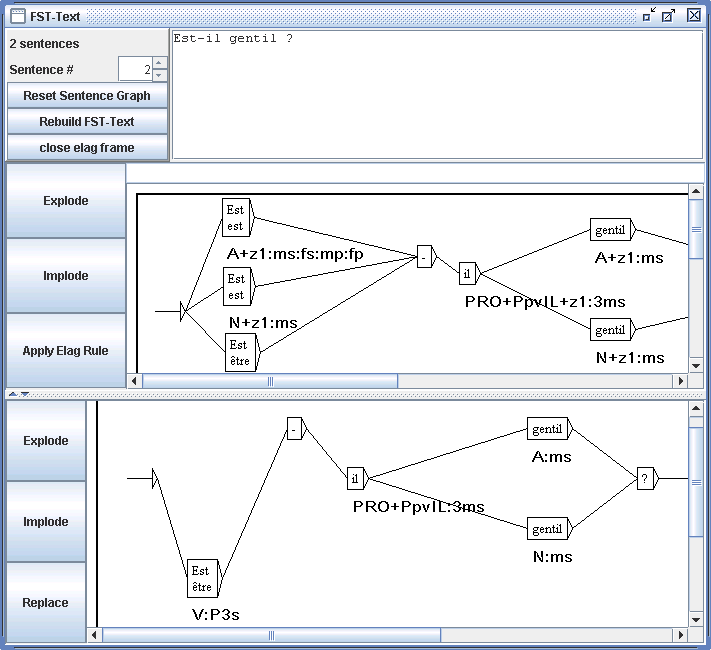
\includegraphics[width=14cm]{resources/img/fig7-15.png}
\caption{Résultat de l’application de la grammaire de la figure~\ref{fig-synchronization-point}\label{fig-est-il}}
\end{center}
\end{figure}

\subsection{Compilation des grammaires ELAG}
\index{Compilation!d'une grammaire ELAG}
Avant de pouvoir être appliquée à un automate de texte, une grammaire ELAG doit être
compilée en un fichier \verb+.rul+. \index{Fichier!\verbc{.rul}} Cette opération s’effectue via
la commande "Elag Rules", dans le menu "Text", qui fait apparaître la fenêtre de la figure
~\ref{fig-elag-rules}.

\begin{figure}[!ht]
\begin{center}
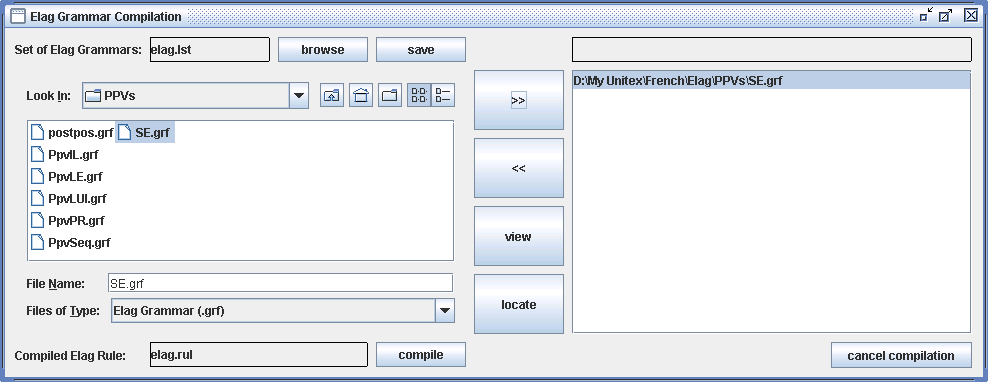
\includegraphics[width=15cm]{resources/img/fig7-16.png}
\caption{Fenêtre de compilation des grammaires ELAG\label{fig-elag-rules}}
\end{center}
\end{figure}

\bigskip
\noindent Si le cadre à droite contient déjà des grammaires que vous ne souhaitez pas utiliser, vous
pouvez les retirer au moyen du bouton "<<". Sélectionnez ensuite votre grammaire dans l’explorateur
de fichiers situé dans le cadre gauche, et cliquez sur le bouton">>" pour l’ ajouter à la liste du
cadre droit. Cliquez alors sur le bouton "Compile". Ceci lancera le programme \verb+ElagComp+
\index{Programmes externes!\verbc{ElagComp}} qui va compiler la grammaire sélectionnée pour créer un
fichier nommé \verb+elag.rul+ par défaut.\index{Fichier!\verbc{.rul}}

\bigskip
\noindent Si vous avez sélectionné votre grammaire dans le cadre droit, vous pouvez rechercher les
motifs qu’elle reconnaît en cliquant sur le bouton "Locate". Cela ouvre la fenêtre "Locate Pattern"
en spécifiant automatiquement un nom de graphe se terminant par
\verb+-conc.fst2+.\index{Fichier!\verbc{-conc.fst2}}
Ce graphe correspond à la partie \textit{si} de la grammaire. Vous pouvez ainsi obtenir les
occurrences du texte sur lesquelles la grammaire s’appliquera.


\bigskip
\noindent NOTE: le fichier \verb+-conc.fst2+ utilisé pour localiser la partie \textit{si}
d’une grammaire est généré lors de la compilation des grammaires ELAG au moyen du bouton
"Compile". Il faut donc avoir d’abord compilé votre grammaire avant d’utiliser la fonction
de recherche du bouton "Locate".


\subsection{Levée d’ambiguïtés}
\index{Levée d’ambiguïtés}
Une fois que vous avez compilé votre grammaire en un fichier \verb+elag.rul+                                                                                  vous pouvez
l’appliquer à l’automate du texte. Dans la fenêtre de l’automate du texte, cliquez sur le bouton 
"Apply Elag Rule". Une boîte de dialogue apparaîtra pour vous demander le nom du fichier \verb+.rul+
à utiliser (voir figure~\ref{fig-text-auto1}). Comme le fichier par défaut est bien \verb+elag.rul+,
cliquez simplement sur "OK". Cela lancera le programme \verb+Elag+\index{Programmes
externes!\verbc{Elag}} qui va effectuer la levée d’ambiguïtés.

\begin{figure}[!ht]
\begin{center}
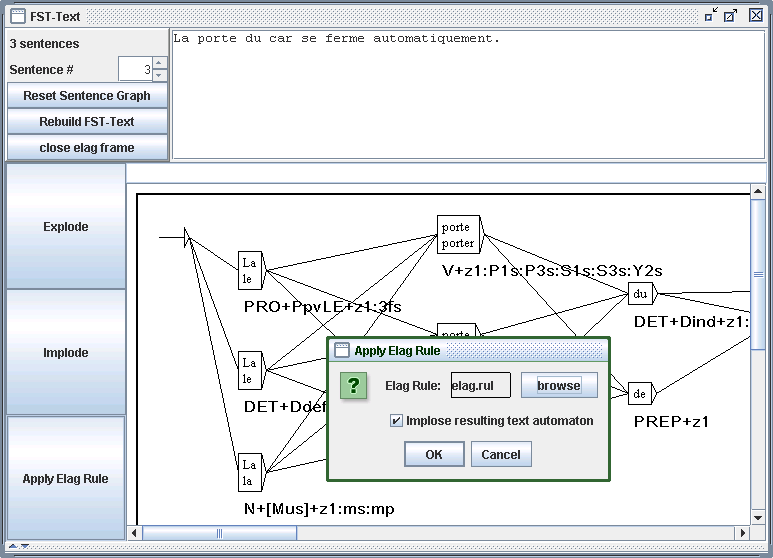
\includegraphics[width=12cm]{resources/img/fig7-17.png}
\caption{Fenêtre de l’automate du texte \label{fig-text-auto1}}
\end{center}
\end{figure}

\bigskip
\noindent Une fois le programme terminé, vous pouvez consulter l’automate résultat en cliquant
sur le bouton "Open Elag Frame" button. Comme on le voit sur la figure~\ref{fig-text-auto2},
la fenêtre est séparée en deux: l’automate d’origine est affiché en haut, et l’automate résultat en bas.


\begin{figure}[!ht]
\begin{center}
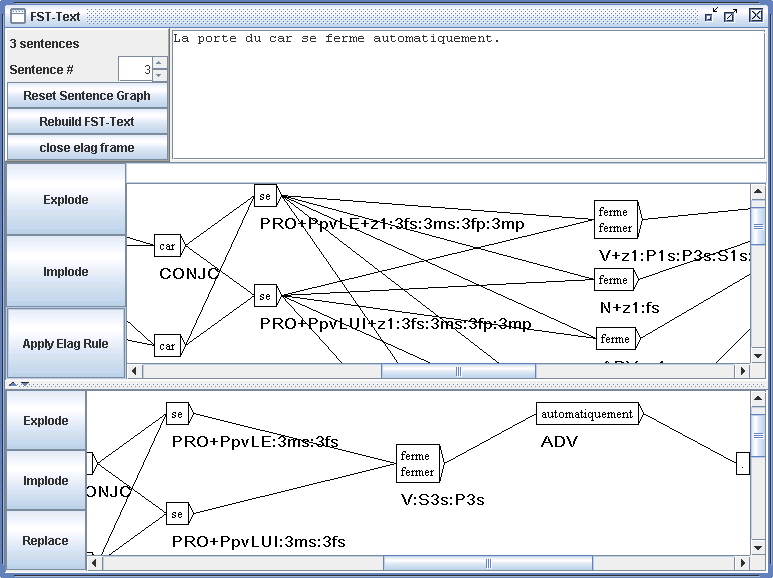
\includegraphics[width=12cm]{resources/img/fig7-18.png}
\caption{Fenêtre de l’automate du texte séparée en deux \label{fig-text-auto2}}
\end{center}
\end{figure}

%\clearpage

\bigskip
\noindent Ne soyez pas étonné si l’automate du bas semble plus compliqué. Cela s’explique par
le fait que les entrées lexicales factorisées\footnote{Ce sont des entrées qui regroupent
 plusieurs interprétations flexionnelles différentes, comme par exemple :
\texttt{\{se,.PRO+PpvLE:3ms:3fs:3mp:3fp\}}.}\index{Factorisation des entrées lexicales}
ont été \textit{explosées} de façon à traiter séparément chaque interprétation flexionnelle.
Pour refactoriser ces entrées, cliquez sur le bouton "Implode". Un clic sur le bouton 
"Explode" vous donne une vue explosée de l’automate du texte.

\bigskip
\noindent Si vous cliquez sur le bouton "Replace", l’automate résultat deviendra le nouvel
automate du texte. Ainsi, si vous utilisez d’autres grammaires, elles s’appliqueront sur l’automate
déjà partiellement désambiguïsé, ce qui permet de cumuler les effets de plusieurs grammaires.



\subsection{Ensembles de grammaires}
\index{Grammaires!collection}
Il est possible de regrouper plusieurs grammaires ELAG en un ensemble de grammaires,
afin de les appliquer en une seule fois. Les ensembles de grammaires ELAG sont décrits dans
des fichiers \verb+.lst+\index{Fichier!\verbc{.lst}}. Ils sont gérés depuis la fenêtre de compilation
des grammaires ELAG (figure~\ref{fig-elag-rules}). Le label en haut à gauche indique le nom de 
l’ensemble courant, par défaut \verb+elag.lst+.C’est le contenu de cet ensemble qui est affiché
dans le cadre droit de la fenêtre.


\bigskip
\noindent Pour modifier le nom de l’ensemble, cliquez sur le bouton "Browse".
Dans la boîte de dialogue qui apparaît alors, choisissez le nom du fichier\verb+.lst+ que vous
voulez donner à votre ensemble.


\bigskip
\noindent Pour ajouter une grammaire à l’ensemble, sélectionnez-la dans l’explorateur de fichiers
du cadre gauche, et cliquez sur le bouton >>.
Pour retirer une grammaire de l’ensemble, sélectionnez-la dans le cadre droit et cliquez
sur le bouton <<.
Une fois que vous avez sélectionné toutes vos grammaires, compilez-les en cliquant sur
le bouton "Compile". Cela créera un fichier \verb+.rul+ portant le nom indiqué en bas à droite (le
	nom du fichier est obtenu en remplaçant l’extension \verb+.lst+ par \verb+.rul+).
\index{Fichier!\verbc{.lst}}\index{Fichier!\verbc{.rul}}

\bigskip
\noindent Vous pouvez maintenant appliquer votre ensemble de grammaires. Comme expliqué
plus haut, cliquez sur le bouton "Apply Elag Rule" dans la fenêtre de l’automate du texte. Quand la boîte de dialogue vous demande le nom du fichier \verb+.rul+ à utiliser, cliquez sur le bouton "Browse" et séletionnez votre ensemble. L’automate résultat est identique à celui qui aurait été obtenu en appliquant successivement chacune des grammaires.

\subsection{Fenêtre de traitement d’ELAG}
\index{Fenêtre de traitement d’ELAG}\index{ELAG!fenêtre de traitement}
Lors de la désambiguïsation, le programme \verb+Elag+ 
\index{Programmes externes!\verbc{Elag}} est lancé dans une fenêtre de traitement qui permet
de voir les messages émis par le programme pendant son exécution.


\bigskip
\noindent Par exemple, lorsque l’automate du texte contient des symboles qui ne correspondent
pas au jeu d’étiquettes d’ELAG (voir section suivante), un message indique la nature de l’erreur
rencontrée. De même, lorsqu’une phrase est rejetée (toutes les analyses possibles
ont été éliminées par les grammaires), un message indique le numéro de la phrase. Cela
permet de localiser rapidement la source des problèmes.


\subsubsection{Évaluation du taux d’ambiguïté}
\index{Évaluation du taux d’ambiguïté}\index{Taux d'ambiguité}
L’évaluation du taux d’ambiguïté ne se base pas uniquement sur le nombre moyen d’interprétations
par mot. Afin d’avoir une mesure plus représentative, le système prend égale-
ment en compte les différentes combinaisons de mots. Durant la levée d’ambiguïtés, le programme 
 \verb+Elag+ calcule le nombre d’analyses possibles dans l’automate du texte avant et après
 modification (cela correspond au nombre de chemins possibles dans l’automate). En se basant sur
 cette valeur, le programme calcule l’ambiguïté moyenne par phrase et par mot. C’est cette dernière
 mesure qui est utilisée pour représenter le taux d’ambiguïtés du texte, car elle ne varie pas avec
 la taille du corpus, ni avec le nombre de phrases de celui-ci. La formule appliquée est:



\bigskip
\begin{center}
	\textit{taux d’ambiguïtés}$=exp^{\frac{log(nombre de chemins)}{longueur du texte}}$
\end{center}

\bigskip \noindent Le rapport entre le taux d’ambiguïtés avant et après l’application des grammaires
donne une mesure de leur efficacité. Toutes ces informations sont affichées dans le fenêtre de
traitement d’ELAG.



\subsection{Description du jeu d’étiquettes}
\label{section-elag-tagset}
\index{Jeu d’étiquettes ELAG}

Les programmes \verb+Elag+ and \verb+ElagComp+  
\index{Programmes externes!\verbc{Elag}}
\index{Programmes externes!\verbc{ElagComp}} nécessitent une description formelle du jeu d’étiquettes
des dictionnaires utilisés. Cette description consiste, grosso modo, en une énumération de toutes
les catégories grammaticales présentes dans les dictionnaires, avec pour
chacune d’elle, la liste des codes syntaxiques et flexionnels qui leur sont associées et une
description de leurs possibles combinaisons. Ces informations sont décrites dans le fichier
nommé \verb$tagset.def$ qui se trouve dans votre répertoire personnel, dans le sous-répertoire de la langue choisie


\subsubsection{\texttt{tagset.def} file}
\index{Fichier!\verbc{tagset.def}}
Voici un extrait du fichier \verb$tagset.def$ utilisé pour le français.

\begin{verbatim}


NAME french

POS ADV
.

POS PRO
flex:
pers   = 1 2 3
genre  = m f
nombre = s p
discr:
subcat = Pind Pdem PpvIL PpvLUI PpvLE Ton PpvPR PronQ Dnom Pposs1s...
complete:
Pind     <genre> <nombre>
Pdem     <genre> <nombre>
Pposs1s  <genre> <nombre>
Pposs1p  <genre> <nombre>
Pposs2s  <genre> <nombre>
Pposs2p  <genre> <nombre>
Pposs3s  <genre> <nombre>
Pposs3p  <genre> <nombre>
PpvIL    <genre> <nombre> <pers>
PpvLE    <genre> <nombre> <pers>
PpvLUI   <genre> <nombre> <pers>      #
Ton      <genre> <nombre> <pers>      # lui, elle, moi
PpvPR                                 # en y
PronQ                                 # ou qui que quoi
Dnom                                  # rien
.

POS A ## adjectifs
flex:
genre  = m f
nombre = s p
cat:
gauche = g
droite = d
complete:
<genre> <nombre>
_  # pour {de bonne humeur,.A}, {au bord des larmes,.A} par exemple
.


POS V
flex:
temps  = C F I J K P S T W Y G X
pers   = 1 2 3
genre  = m f
nombre = s p
complete:
W
G
C <pers> <nombre>
F <pers> <nombre>
I <pers> <nombre>
J <pers> <nombre>
P <pers> <nombre>
S <pers> <nombre>
T <pers> <nombre>
X 1 s   # eusse dusse puisse fusse (-je)
Y 1 p
Y 2 <nombre>
K <genre> <nombre>
.
\end{verbatim}

\bigskip
\noindent Le symbole  \verb$#$ indique que le reste de la ligne est en commentaire.
Un commentaire peut apparaître à n’importe quel endroit dans le fichier. Le fichier
commence toujours par le mot \verb$NAME$, suivi par un identifiant (\texttt{french}, dans l’exemple).
La suite du fichier est constituée de sections \verb$POS$ (pour Part-Of-Speech, partie du discours),
une pour chaque catégorie grammaticale. Chaque section décrit la structure des étiquettes des
entrées lexicales appartenant à la catégorie grammaticale concernée. Chaque section se compose de 4
parties qui sont toutes optionnelles:


\begin{itemize}
  \item \verb$flex$\index{\verbc{flex}}: cette partie énumère les codes flexionnels
 relatifs à la catégorie grammaticale. Par exemple, les codes \verb$1,2,3$ qui dénotent
 la personne de l’entrée, sont des codes pertinents pour les pronoms mais pas pour les adjectifs. 
 Chaque ligne décrit un attribut flexionnel (genre, temps, etc), et est composée du nom
 de l’attribut, suivi du signe \verb$=$ et des valeurs qu’il peut prendre;
 Par exemple, la ligne suivante déclare un attribut $pers$ pouvant prendre les valeurs
 $1$, $2$ or $3$:

\begin{verbatim}
pers = 1 2 3
\end{verbatim}

\item \verb$cat$\index{\verbc{cat}}: cette partie déclare les attributs syntaxiques
et sémantiques qui peuvent être attribués
aux entrées appartenant à la catégorie grammaticale concernée. Chaque ligne décrit
un attribut et les valeurs qu’il peut prendre. Les codes déclarés pour un même attribut
doivent être exclusifs les uns des autres. Autrement dit, une entrée ne peut pas
prendre plus d’une valeur pour un même attribut.
En revanche, il peut exister des étiquettes ne prenant aucune valeur pour un attribut donné.
Par exemple, pour définir l’attribut \verb$niveau_de_langue$ pouvant prendre les valeurs 
\verb$z1$, \verb$z2$ et \verb$z3$, on écrira la ligne suivante:


\begin{verbatim}
niveau_de_langue = z1 z2 z3
\end{verbatim}

%but this attribute is not necessarily present in all words.
mais cet attribut n'est pas forcément présent pour tous les mots.

\item \verb$discr$\index{\verbc{discr}}: cette partie est constituée de la déclaration
d’un unique attribut. La syntaxe est la même que dans la partie \verb$cat$ et l’attribut
décrit ici ne doit pas y être répété. Cette partie permet de diviser la catégorie grammaticale
en sous-catégories \textit{discriminantes} dans lesquelles les entrées ont des attributs
flexionnels similaires. Pour les pronoms par exemple, une indication de personne est attribuée
aux entrées appartenant à la sous-catégorie des pronoms personnels mais non aux pronoms relatifs.
Ces dépendances sont décrites dans la partie \verb$complete$;

\item \verb$complete$\index{\verbc{complete}}: Dans cette partie est explicité l’étiquetage
morphologique des mots appartenant à la catégorie grammaticale courante. Chaque ligne décrit
une combinaison valide de codes flexionnels en fonction de leur sous catégorie discriminante
(si une telle catégorie a été déclarée). Lorsqu’un nom d’attribut apparaît entre angles
(\verb$<$ et \verb$>$), cela signifie que n’importe quelle valeur de cet attribut peut convenir.
 Il est également possible de déclarer qu’une entrée ne prend aucun trait flexionnel au moyen d’une
 ligne ne contenant que le caractère \verb$_$ (underscore).\index{\verbc{_}} Ainsi par exemple, si
 nous considérons les lignes suivantes extraites de la section concernant la description des verbes :



\begin{verbatim}
W
K <genre> <nombre>
\end{verbatim}

Elles permettent de déclarer que les verbes à l’infinitif (dénoté par le code
\verb$W$) n’ont pas d’autres traits flexionnels positionnés tandis que les formes
à participe passé (code \verb$K$) sont également attribuées d’un genre et d’un nombre.

\end{itemize}

\subsubsection{Description des codes flexionnels}
\index{Codes flexionnels}
La principale fonction de la partie \verb$discr$ est de diviser les étiquettes en sous-catégories
ayant un comportement morphologique similaire. Ces sous-catégories sont ensuite utilisées
pour faciliter l’écriture de la partie \verb$complete$.

\bigskip
\noindent Pour la lisibilité des grammaires ELAG, il est souhaitable que les éléments d’une même
sous-catégorie aient tous le même comportement flexionnel; dans ce cas, la partie \verb$complete$ 
est composée d’une seule ligne par sous-catégorie.

Considérons par exemple les lignes suivantes, extraites de la description des pronoms:

\begin{verbatim}
Pdem  <genre> <nombre>
PpvIl <genre> <nombre> <pers>
PpvPr
\end{verbatim}

\bigskip
\noindent Ces lignes signifient:
\begin{itemize}
  \item tous les pronoms démonstratifs (\verb$PRO+Pdem>$) ont des indications de 
  	  genre et de nombre, et aucune autre ;
  \item les pronoms personnels nominatifs (\verb$<PRO+PpvIl>$) sont étiquetés
  	  morphologiquement par une personne, un genre et nombre ;
  \item les pronoms prépositionnels (\textit{en}, \textit{y}) n’ont aucun trait flexionnel.
\end{itemize}

\bigskip
\noindent Toutes les combinaisons des traits flexionnels et discriminants qui apparaissent dans
les dictionnaires doivent être décrites dans le fichier \verb$tagset.def$;
\index{Fichier!\verbc{tagset.def}} faute de quoi les entrées correspondantes seront rejetées par
ELAG.


\bigskip
\noindent Dans le cas où des mots d’une même sous-catégorie diffèrent par leurs traits flexionnels,
il est nécessaire d’écrire plusieurs lignes dans la partie \verb$complete$. L’inconvénient de cette
méthode de description est qu’il devient difficile de faire la distinction entre de tels mots
dans une grammaire ELAG.


\bigskip
\noindent Si l’on considère la description donnée précédemment en exemple, certains adjectifs du
français prennent un genre et un nombre, alors que d’autres n’ont aucun trait flexionnel.
C’est par exemple le cas de séquences figées comme \textit{de bonne humeur} qui ont un comportement
syntaxique très proche de celui des adjectifs.


\bigskip
\noindent De telles séquences ont ainsi été intégrées dans le dictionnaire du français en tant
qu’adjectifs invariables et donc sans trait flexionnel. Le problème est que si l’on veut faire
référence exclusivement à ce type d’adjectifs dans une grammaire de désambiguïsation, le symbole
 \verb$<A>$ ne convient pas, puisqu’il donnera tous les adjectifs.
Pour contourner cette difficulté, il est possible de nier un attribut flexionnel, en écrivant
le caractère \verb$@$ juste avant une des valeurs possibles pour cet attribut. Ainsi, le symbole
\verb$<A:@m@p>$ reconnaît tous les adjectifs qui n’ont ni genre ni nombre. A l’aide de cet opérateur, il 
est maintenant possible d’écrire des grammaires comme celles de la figure~\ref{fig-NA}, qui 
imposent l’accord en genre et en nombre entre un nom et l’adjectif qui le suit
\footnote{   Cette grammaire n’est pas complètement correcte, car elle élimine par exemple l’analyse correcte de la
phrase : \textit{J'ai re\c{c}u des coups de fil de ma m\`ere hallucinants.}}.
Cette grammaire conservera l’analyse correcte de phrases comme: \textit{Les
personnes de bonne humeur m'insupportent}.

\bigskip
\noindent Il est toutefois recommandé de limiter l’usage de l’opérateur @, car cela nuit à la lisibilité
des grammaires. Il est préférable de distinguer les étiquettes qui acceptent différentes com-
binaisons flexionnelles au moyen de sous-catégories discriminantes définies dans la partie
\verb$discr$.

\begin{figure}[!ht]
\begin{center}
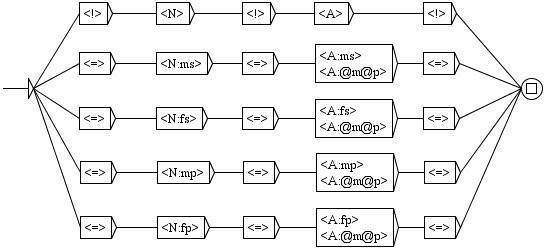
\includegraphics[width=12cm]{resources/img/fig7-19.png}
\caption{Grammaire ELAG vérifiant l’accord en genre et en nombre entre un nom et l’adjectif qui le suit
\label{fig-NA}}
\end{center}
\end{figure}

\subsubsection{Codes optionnels}
Les codes syntaxiques et sémantiques optionnels sont déclarés dans la partie cat. Ils
peuvent être utilisés dans les grammaires ELAG comme les autres codes. La différence est
que ces codes n’interviennent pas pour décider si une étiquette doit être rejetée comme
invalide ou non, lors du chargement de l’automate du texte.


\bigskip
\noindent Ce sont des codes facultatifs, qui sont indépendants des autres codes, 
comme par exemple l’attribut de niveau de langue (\verb$z1$, \verb$z2$ or \verb$z3$). 
De la même manière que pour les codes flexionnels, il est également possible de nier
un attribut flexionnel en écrivant le caractère \verb$!$ juste avant le nom de l’attribut.
Ainsi, avec notre fichier d’exemple, le symbole \verb$<A!gauche:f>$ reconnaît tous les
adjectifs au féminin qui ne possèdent pas le code \verb$gauche$,\footnote{Ce code indique 
que l’adjectif doit apparaître à gauche du nom auquel il se rapporte, comme c’est le cas
pour \textit{bel}.}.

\bigskip
\noindent Tous les codes qui ne sont pas déclarés dans le fichier
\verb$tagset.def$\index{Fichier!\verbc{tagset.def}} sont ignorés par ELAG. Si une entrée de
dictionnaire contient un tel code, ELAG produira un avetissement et retirera le code de l’entrée.


\bigskip
\noindent En conséquence, si deux entrées concurrentes ne différaient dans l’automate du texte
d’origine que par des codes non déclarés, ces entrées deviendront indistinguables par le programme
et seront donc unifiées en une seule entrée dans l’automate résultat.


\bigskip
\noindent Ainsi, le jeu d’étiquettes décrit dans le fichier \verb$tagset.def$                                                                                peut suffire à
réduire l’ambiguïté, en factorisant des mots qui ne diffèrent que par des codes non déclarés
et ceci indépendamment des grammaires appliquées.


\bigskip
\noindent Par exemple, dans la version la plus complète du dictionnaire du français, chaque emploi
distinct d’un verbe est caractérisé par une référence vers la table du lexique-grammaire qui
le caractérise. Nous avons considéré jusqu’à présent que ces informations relèvent plus de
la syntaxe que de l’analyse lexicale et nous ne les avons donc pas intégrées dans la description
du jeu d’étiquettes. Celle-ci sont donc automatiquement éliminées lors du chargement de
l’automate du texte, ce qui réduit son taux d’ambiguïtés.


\bigskip
\noindent Afin de bien distinguer les effets liés au jeu d’étiquettes de ceux des grammaires
ELAG, il est conseillé de procéder à une étape préalable de normalisation de l’automate
du texte avant de lui appliquer les grammaires de désambiguïsation. Cette normalisation
s’effectue en appliquant à l’automate du texte une grammaire n’imposant aucune contrainte,
comme celle de la figure~\ref{fig-elag-norm}. Notez que cette grammaire est normalement présente
dans la distribution d’Unitex et pré-compilée dans le fichier
\verb+norm.rul+.\index{\verbc{norm.rul}}\index{Fichier!\verbc{norm.rul}}

\begin{figure}[!ht]
\begin{center}
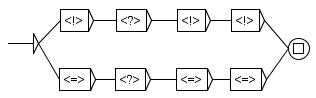
\includegraphics[width=9cm]{resources/img/fig7-20.png}
\caption{Grammaire ELAG n’exprimant aucune contrainte\label{fig-elag-norm}}
\end{center}
\end{figure}

\bigskip
\noindent Le résultat de l’application de cette grammaire est que l’automate d’origine est nettoyé
de tous les codes qui ne sont, soit pas décrits dans le fichier \verb$tagset.def$,
\index{Fichier!\verbc{tagset.def}} soit non conformes
à cette description (à cause de catégories grammaticales inconnues ou de combinaisons invalides 
de traits flexionnels). En remplaçant alors l’automate du texte par l’automate ainsi
normalisé, on peut être sûr que les modifications ultérieures de l’automate seront 
uniquement dues aux effets des grammaires ELAG.


\subsection{Optimiser les grammaires}
\index{Optimiser les grammaires ELAG}
La compilation des grammaires effectuée par le programme \verb+ElagComp+
\index{Programmes externes!\verbc{ElagComp}} consiste à constr-uire un automate dont le langage est
l’ensemble des séquences d’entrées lexicales (ou interprétations lexicales d’une phrase) qui ne sont
pas rejetées par les grammaires. Cette tâche est complexe et peut prendre beaucoup de temps, il est
toutefois possible de l’accélérer sensiblement en observant certains principes lors de l’écriture
des grammaires.


\subsubsection{Limiter le nombre de branches \textit{alors}}
\noindent Il est recommandé de réduire au minimum le nombre de parties \textit{alors} d’une grammaire.
Cela peut réduire considérablement le temps de compilation des grammaires. Le plus souvent, 
une grammaire possédant beaucoup de parties \textit{alors} peut être réécrite avec une ou
deux parties \textit{then} sans perte de lisibilité. C’est par exemple le cas de la grammaire 
de la figure ~\ref{fig-NA-bad} qui impose une contrainte entre un verbe et le pronom qui le suit.

\begin{figure}[!ht]
\begin{center}
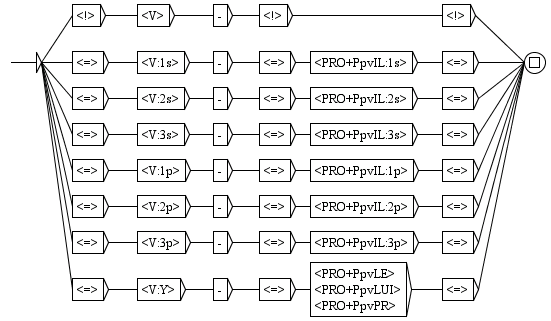
\includegraphics[width=15cm]{resources/img/fig7-21.png}
\caption{Grammaire ELAG vérifiant l’accord entre verbe et pronom\label{fig-NA-bad}}
\end{center}
\end{figure}

\bigskip
\noindent Comme on peut le voir sur la figure~\ref{fig-NA-good}, on peut écrire une grammaire
équivalente en factorisant toutes les parties \textit{alors} en une seule. Les deux grammaires auront exactement le même effet sur l’automate du texte, mais la seconde sera compilée beaucoup plus rapidement.


\begin{figure}[!ht]
\begin{center}
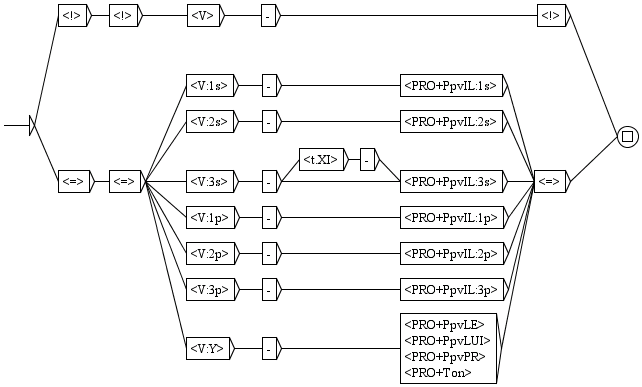
\includegraphics[width=15cm]{resources/img/fig7-22.png}
\caption{Grammaire ELAG optimisée vérifiant l’accord entre verbe et pronom\label{fig-NA-good}}
\end{center}
\end{figure}


\subsubsection{Utilisation des symboles lexicaux}
\index{Symboles!lexicaux}
\noindent Il vaut mieux n’utiliser les lemmes que lorsque c’est absolument nécessaire. Cela est
particulièrement vrai pour les mots grammaticaux, lorsque leurs sous-catégories portent
presque autant d’information que les lemmes eux-mêmes. Si vous utilisez malgré tout un
lemme dans un symbole, il est recommandé de préciser le plus possible ses traits syntaxiques, 
sémantiques et flexionnels.
Par exemple, avec les dictionnaires fournis pour le français, il est préférable de remplacer des 
symboles comme \verb$<je.PRO:1s>$, \verb$<je.PRO+PpvIL:1s>$ et \verb$<je.PRO>$
par le symbole \verb$<PRO+PpvI1:1s>$. En effet, tous ces symboles sont identiques dans la 
mesure où ils ne peuvent reconnaître que l’unique entrée de dictionnaire 
\verb${je,PRO+PpvIL:1ms:1fs}$. Cependant, comme le programme ne peut pas déduire automatiquement
cette information, si l’on ne précise pas tous ces traits, le programme considérera en vain des 
étiquettes non existantes telles \verb$<je.PRO:3p>$, \verb$<je.PRO+PronQ>$ etc. en vain.


\section{Linéarisation de l'automate du texte avec le taggeur}
\label{section-linearization}
Par défaut, l'automate du texte contient de nombreux chemins étiquetés en raison de l'ambiguïté
lexicale. Le processus de linéarisation consiste à choisir un chemin unique, une séquence
d'étiquettes avec une étiquette par token et de supprimer les autres. 
Le résultat est un automate du texte avec un seul chemin (voir section \ref{section-linear-text}
pour convertir un automate linéaire en un texte linéaire). Le choix du chemin dépend de son score.
Le chemin avec le meilleur score est choisi et les autres supprimés
Le score d'un chemin est calculé par un modèle statistique entrainé sur un corpus annoté.
Ce modèle utilise des fichiers de données du taggeur produites par le programme 
TrainingTagger (vour section \ref{section-TrainingTagger}). 
Par exemple, vous pouvez voir figure \ref{fig7-linearize2}, l'automate du texte original sur la
phrase \textit{Les insectes nuisibles envahissent la maison}. L'automate du texte après
linéarisation est celui de la figure \ref{fig7-linearize3}.

\begin{figure}[!ht]
\begin{center}
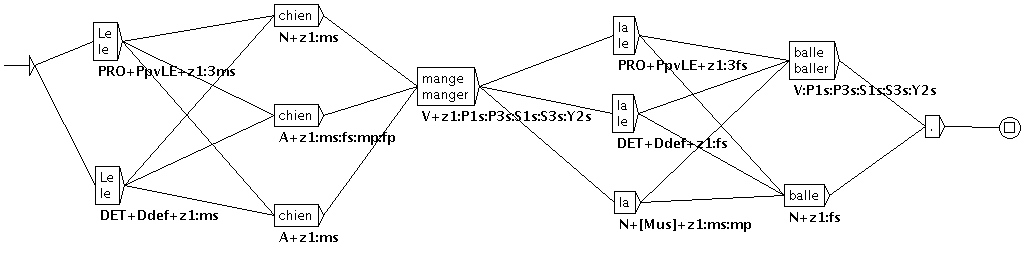
\includegraphics[width=16cm]{resources/img/fig7-linearize2.png}
\caption{Automate du texte de \textit{Les insectes nuisibles envahissent la maison.}\label{fig7-linearize2}}
\end{center}
\end{figure}

\begin{figure}[!ht]
\begin{center}
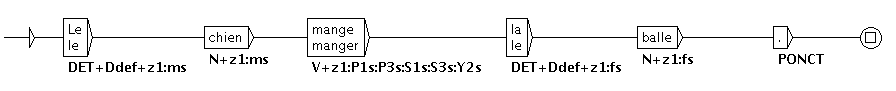
\includegraphics[width=16cm]{resources/img/fig7-linearize3.png}
\caption{Automate du texte linéarisé\label{fig7-linearize3}}
\end{center}
\end{figure}

\subsection{Compatibilité du jeu d'étiquettes}
\label{section-linearization-tagset}

Le jeu d'étiquettes du taggeur est identique à celui du corpus d'entrainement ou en est une variante
(voir ci-dessous). Toutefois, pour utiliser le taggeur sur l'automate du texte, on doit faire
attention au jeu d'étiquettes et à la morphologie. Le jeu d'étiquettes du modèle doit être identique
à celui de l'automate du texte. Par exemple, si le modèle statistique a été calculé avec les
étiquettes \verb+DET+ pour les mots \verb+the+, l'étiquette correspondante dans le texte doit être
\verb+DET+. Unitex dispose d'une fonctionnalité qui permet de changer la forme des mots du texte, par
exemple pour normaliser \verb+doesn't+ en \verb+does not+. Appliquer des graphes de remplacement ou
de normalisation peut entrainer des modifications de la forme des mots. Si un tel traitement a été
appliqué au texte, il doit avoir été appliqué également au corpus d'entrainement. Si ces règles ne
sont pas respectées, le taggeur pourrait être incapable de trouver le chemin souhaité dans
l'automate du texte.

\bigskip
\noindent Le programme TrainingTagger produit deux variantes de taggeur. Le premier supprime des
transitions sur la base de codes gramaticaux, sémantiques, syntaxiques et flexionnels
(par exemple, \verb$the.DET+Ddef:s$ au lieu de \verb$the.DET+Ddef:p$). 
Le second supprime les transitions sur la base de codes gramaticaux, sémantiques et syntaxiques
(\verb$that.DET+Ddem$ au lieu de \verb$that.PRO+Pdem$). Ce traitement accélère l'entrainement et les
informations flexionnelles ne sont plus nécessaires pour toutes les
applications.

\subsection{Utilisation du Tagger}
Pour linéariser l'automate du texte, vous devez choisir l'option "Linearize with the Tagger" dans la
fenêtre de configuration pour construire l'automate du texte (cf. figure \ref{fig7-linearize1}).
Avec cette option, le programme linéarise chaque phrase de l'automate. Vous devez également
sélectionner le fichier de données du taggeur (avec l'extension ".bin") en cliquant sur le bouton
"Set". Le fichier de données du taggeur suffixé par "morph" est la première variante (avec les codes
flexionnels) et celle suffixée par "cat" est la seconde (sans codes flexionnels). Si vous utilisez
les données de type "morph", vous devez également cliquer sur "Normalize accordind to Elag
tagset.def" (pour plus de  détails, voir section \ref{section-Tagger} au sujet du programme
\verb+Tagger+).

\begin{figure}[!ht]
\begin{center}
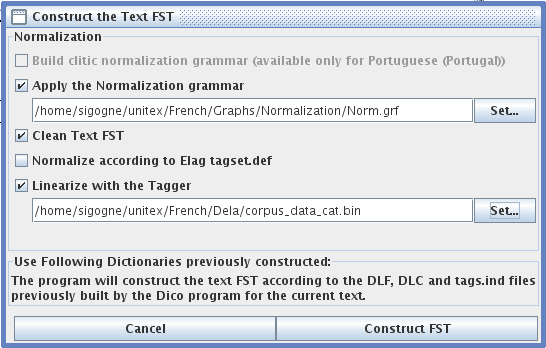
\includegraphics[width=13cm]{resources/img/fig7-linearize1.png}
\caption{Configuration de la linéarisation de l'automate du texte\label{fig7-linearize1}}
\end{center}
\end{figure}

\bigskip
\noindent Par exemple, l'automate du texte, de la figure \ref{fig7-linearize3}, est la sortie de la  linéarisation de l'automate du texte de la figure \ref{fig7-linearize2} avec la version "cat".
La linéarisation de l'automate avec la version "morph" se trouve figure \ref{fig7-linearize4}.

\begin{figure}[!ht]
\begin{center}
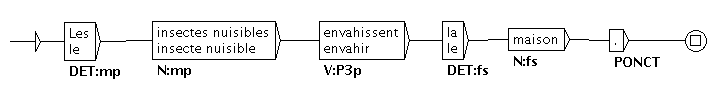
\includegraphics[width=16cm]{resources/img/fig7-linearize4.png}
\caption{L'automate du texte linéarisé avec les données de type "morph"\label{fig7-linearize4}}
\end{center}
\end{figure}

\subsection{Création d'un nouveau taggeur}
Pour créer un nouveau taggeur pour votre langue, vous devez lancer le programme TrainingTagger sur
votre propre corpus annoté. Le format du corpus annoté est décrit dans \ref{section-corpus-file}.
Comme nous le signalions à la section \ref{section-linearization-tagset}, 
vous devez faire attention au jeu d'étiquettes et à la morphologie. Avant de calculer un modèle
statistique, vous devez décider quels dictionnaires et graphes de normalisation vous utiliserez pour
construire l'automate du texte. Puis, vous devrez modifier le corpus annoté si la forme des mots ou
le jeu d'étiquettes ne sont pas identiques. Par exemple, si le graphe de  normalisation transforme
le mot \verb+jusqu'+ en \verb+jusque+, le mot correspondant dans le  corpus annoté doit
être\verb+jusque+. 

\bigskip
\noindent Un taggeur pour le français est fourni avec Unitex. Il a été créé avec un corpus annoté 
composé d'étiquettes dépourvues de codes sémantiques et syntaxiques.



\section{Manipulation de l’automate du texte}

\subsection{Affichage des automates de phrases}
\label{section-displaying-sentence-automata}
Comme nous l’avons vu précédemment, l’automate d’un texte est en réalité l’ensemble
des automates des phrases de ce texte. Cette structure peut être représentée grâce au format
\verb+.fst2+, utilisé pour représenter les grammaires compilées.\index{Fichier!\verbc{.fst2}} 
Cependant, ce format ne permet pas d’afficher directement les automates de phrases. Il
faut donc utiliser un programme \verb+Fst2Grf+\index{\verbc{Fst2Grf}}\index{Programmes
externes!\verbc{Fst2Grf}} pour convertir un automate de phrase en un graphe pour qu’il 
puisse être affiché. Ce programme est appelé automatiquement quand
vous sélectionnez une phrase pour générer le fichier \verb+.grf+.
\index{Fichier!\verbc{.grf}}

\bigskip
\noindent Les fichiers \verb+.grf+ générés ne sont pas interprétés de la même manière
que les fichiers \verb+.grf+ qui représentent des graphes construits par l’utilisateur. 
En effet, dans un graphe normal, les lignes d’une boîte sont séparées par le symbole \verb$+$.
Dans un graphe de phrase, chaque boîte est, soit une unité lexicale sans étiquette, soit une 
entrée de dictionnaire encadrée par des accolades. Si la boîte ne contient qu’une unité sans 
étiquette, celle-ci apparaît seule dans la boîte. Si la boîte contient une entrée de dictionnaire, 
la forme fléchie est affichée, suivie de sa forme canonique si celle-ci est différente. 
Les informations grammaticales et flexionnelles sont affichées sous la boîte, comme dans les transductions.



\bigskip
\noindent La figure~\ref{fig-first-sentence-Ivanhoe} montre le graphe obtenu pour 
la première phrase \textit{Ivanhoe}. Les mots \verb+Ivanhoe+,
\verb+Walter+ et \verb+Scott+ sont considérés comme des mots inconnus. Le mot \verb+by+
correspond à deux entrées dans le dictionnaire. Le mot \verb+Sir+ correspond également à 
deux entrées du dictionnaire, mais comme la forme canonique de ces entrées est
\verb+sir+, elle est affichée puisqu’elle diffère de la forme fléchie par une minuscule.


\begin{figure}[!ht]
\begin{center}
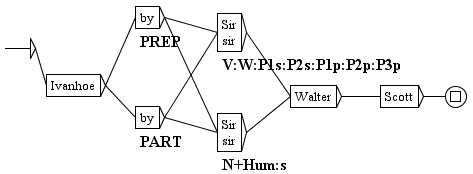
\includegraphics[width=11cm]{resources/img/fig7-23.png}
\caption{Automate de la première phrase \textit{Ivanhoe}\label{fig-first-sentence-Ivanhoe}}
\end{center}
\end{figure}

\subsection{Modifier manuellement l’automate du texte}
Il est possible de modifier manuellement les automates de phrase, sauf ceux qui appa-
raissent dans le cadre réservé à ELAG (cadre du bas). On peut modifier ou supprimer des
boîtes ou des transitions (voir figure~\ref{fig-modified-sentence-automaton}).

\begin{figure}[!ht]
\begin{center}
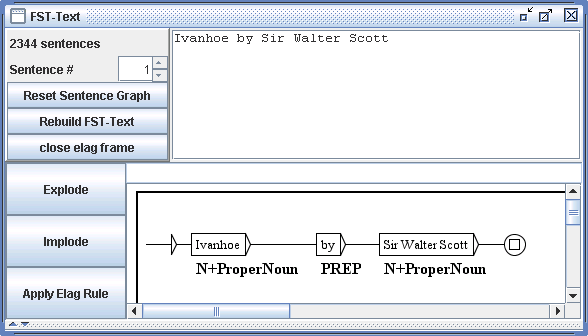
\includegraphics[width=15cm]{resources/img/fig7-24.png}
\caption{Automate de phrase modifié\label{fig-modified-sentence-automaton}}
\end{center}
\end{figure}

\bigskip
\noindent Lorsqu’un graphe est modifié, il est sauvegardé dans le répertoire
du texte sous le nom \verb+sentenceN.grf+, où $N$ représente le numéro de la phrase,
mais cette opération ne modifie pas l'automate global du texte.
On peut donc annuler les modifications faites manuellement et réinitialiser l’automate de cette phrase
en cliquant sur le bouton "Reset Sentence Graph".

\bigskip
\noindent Lorsqu’on sélectionne une phrase, si un graphe modifié existe pour cette phrase,
Unitex l'affiche.

\bigskip
\noindent Après avoir édité des automates de phrases, on peut sauvegarder ses modifications
manuelles dans l’automate global du texte. Pour cela, on clique sur le bouton "Rebuild FST-Text". Toutes les phrases
pour lesquelles des modifications ont été faites sont alors remplacées dans l’automate du
texte par leur version modifiée. Le nouvel automate du texte est ensuite rechargé automatiquement.

\bigskip
\noindent Lors de la construction de l’automate d’un texte (\ref{construction-text-automaton}), toutes les
modifications manuelles sauvegardées dans l'automate du texte sont annulées.


%%%%%%%%%%%%%%%%
\subsubsection{Levée manuelle des ambiguïtés}
L’automate du texte peut contenir de nombreux chemins étiquetés en raison de l'ambiguïté lexicale.
Vous pouvez soit lever les ambiguités avec des grammaires ELAG, soit sélectionner manuellement les chemins
corrects pour l'un ou tous les graphes de l'automate de phrase. Vous devez pour cela effectuer un
clic droit sur la boîte que vous voulez garder lorsque plusieurs boîtes avec différentes étiquettes
sont proposées. Les bords de la boîte sélectionnée deviendront plus gras tandis que les autres
boîtes apparaîtront grisées (voir figure~\ref{fig-manually-resolve-ambiguities}).

\begin{figure}[!ht]
\begin{center}
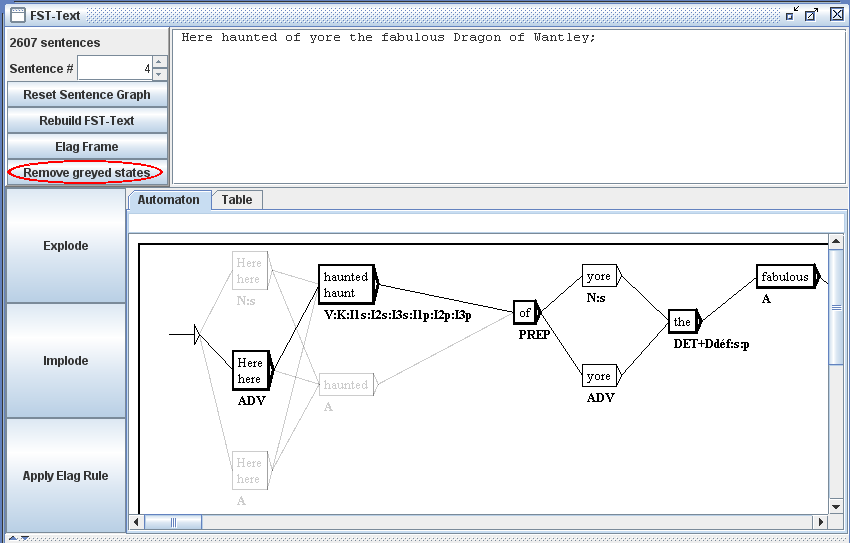
\includegraphics[width=15cm]{resources/img/fig7-24b.png}
\caption{Levée manuelle d'ambiguités dans l'automate de
phrases\label{fig-manually-resolve-ambiguities}}
\end{center}
\end{figure} 

\bigskip
\noindent Vous pouvez alors cliquer sur le bouton "Remove greyed states" pour ne garder que les
boîtes sélectionnées (figure~\ref{fig-removed-ambiguities}).

\begin{figure}[!ht]
\begin{center}
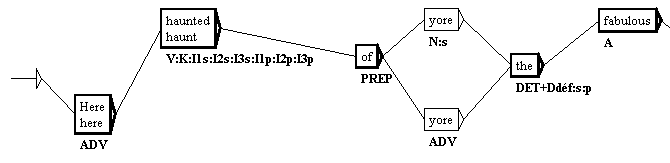
\includegraphics[width=11cm]{resources/img/fig7-24c.png}
\caption{Suppression de boîtes ambiguës dans l'automate de phrase
\label{fig-removed-ambiguities}}
\end{center}
\end{figure}

\bigskip
\noindent
%\subsection{Configuration d'affichage}


%%%%%%%%%%%%%%%

\subsection{Paramètres de présentation}
Les automates de phrase sont soumis aux mêmes options de présentation que les graphes.
Ils partagent les mêmes couleurs et polices de caractères, ainsi que l’utilisation de l’effet
d’antialiasing. Pour configurer l’apparence des automates de phrase, vous devez modifier
la configuration générale en cliquant sur "Preferences..." dans le menu "Info". Pour plus de
détails, reportez-vous à la section~\ref{section-display-fonts-colors}.

\bigskip
\noindent Vous pouvez également imprimer un automate de phrase en cliquant sur "Print..." dans
le menu "FSGraph" ou en appuyant sur <Ctrl+P>. Assurez-vous que le paramètre d’orientation de 
l’imprimante est bien réglé sur le mode paysage. \index{Impression!automate de phrase}
Pour régler ce paramètre, cliquez sur "Page Setup" dans le menu "FSGraph".


\section{Convertir l’automate du texte en texte linéaire}
\label{section-linear-text}
\index{Automate!du texte!conversion en texte linéaire}
    Si l’automate du texte ne contient plus la moindre ambiguïté, il est possible de construire
un fichier texte correspondant à l’unique chemin représenté par cet automate. Pour cela,
allez dans le menu "Text" et cliquez sur "Convert FST-Text to Text...". La fenêtre de la figure
~\ref{fig-linearization-configuration} vous permet alors de définir le fichier texte de sortie.

\begin{figure}[!ht]
\begin{center}
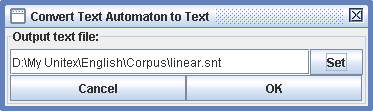
\includegraphics[width=10cm]{resources/img/fig7-25.png}
\caption{Choix du fichier de sortie pour la linéarisation de l’automate du texte\label{fig-linearization-configuration}}
\end{center}
\end{figure}

\bigskip
\noindent Si l’automate n’est pas complètement linéaire, un message d’erreur vous indiquera
le numéro de la première phrase contenant une ambiguïté. Sinon, le programme \verb+Tfst2Unambig+ 
construira le fichier de sortie selon les principes suivants:

\index{Programmes externes!\verbc{Tfst2Unambig}}\index{\verbc{Tfst2Unambig}}
\begin{itemize}
  \item le fichier de sortie contient une ligne par phrase;
  \item toutes les phrases sauf la dernière sont terminées par \verb+{S}+;
  \item pour chaque boîte, le programme écrit son contenu suivi par un espace.
\end{itemize}

\begin{figure}[!ht]
\begin{center}
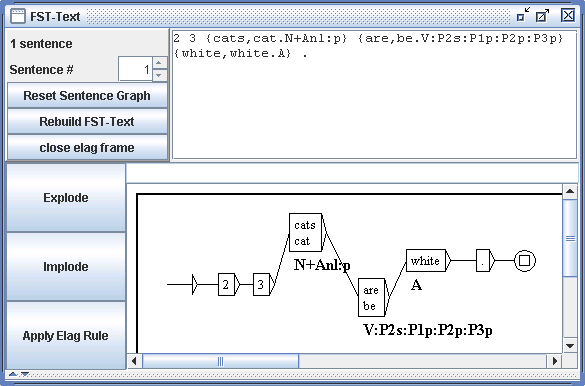
\includegraphics[width=12cm]{resources/img/fig7-26.png}
\caption{Exemple d’automate de texte linéaire\label{fig-linear-automaton}}
\end{center}
\end{figure}

\bigskip
\noindent NOTE : la gestion des espaces est entièrement laissée à l’utilisateur. 
Ainsi, si le texte d’origine est celui de l’automate de phrase de la figure 
\ref{fig-linear-automaton}, le texte produit sera:

\begin{verbatim}
2 3 {cats,cat.N+Anl:p} {are,be.V:P2s:P1p:P2p:P3p} {white,white.A} .
\end{verbatim}


\section{Recherche de motifs dans l'automate du texte}
\label{section-locate-tfst}
Le programme \verb+LocateTfst+ d'Unitex peut effectuer des recherches sur l'automate du texte.
Les principaux avantages sont que vous pouvez:
\begin{itemize}
\item bénéficier de la suppression de l'ambiguité;
\item bénéficier de l'application de grammaire de normalisation (voir ci-dessous);
    \item travailler à plusieurs niveaux morphologiques (mots composés, mots simples morphèmes).
    	    C'est particulièrement intéressant car vous pouvez facilement manipuler les langues agglutinantes comme le coréen (pour le coréen, voir
    section \ref{section-korean}).
\end{itemize}

 
\bigskip
\noindent Les règles sont très proches de celles qui s'appliquent lors des recherches avec
\verb+Locate+. Voici les différences:

\begin{itemize}
    \item vous ne pouvez pas mémoriser des séquences dans des variables, comme avec \verb+Locate+
    	    (voir figure \ref{fig-context6}, page \pageref{fig-context6})
    \item vous ne pouvez pas reconnaître des choses qui ne sont pas l'automate du texte:
    si l'automate du texte contient seulement l'étiquette d'un mot composé, mais pas des
    mots simples qu'il renferme, vous ne pourrez pas reconnaître les mots simples.
    Par exemple, dans la phrase de l'automate de la figure~\ref{fig7-locatetfst1},
    il est impossible reconnaître \verb+soixante+ ou \verb+huit+, puisque ces chemins n'existent pas.
    
\begin{figure}[!ht]
\begin{center}
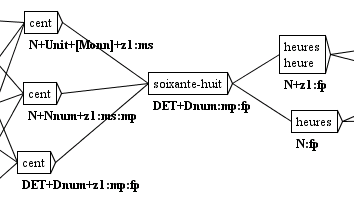
\includegraphics[width=9cm]{resources/img/fig7-locatetfst1.png}
\caption{Phrase de l'automate qui ne reconnaît pas le motif
\textit{huit}\label{fig7-locatetfst1}}
\end{center}
\end{figure}

\item les séquences reconnues peuvent être différentes de celles apparaissant dans les concordances.
	En fait, l'automate du texte peut contenir des étiquettes qui ne correspondent pas au texte
	brut d'entrée, en particulier lorsqu'une grammaire de normalisation a été appliquée.
	Par exemple, si vous recherchez le motif \verb+<le.DET>+ dans l'automate du texte de
	\textit{80jours}, vous obtenez 7703 matches, tandis que \verb+Locate+ n'en trouve que 5763.
	Ceci provient du fait que quelques mots ont été normalisés, comme \verb+au+
	$\rightarrow$ \verb+à le+ ou \verb+du+ $\rightarrow$\verb+de le+.
	Ainsi, quand vous cherchez \verb+<le.DET>+, \verb+LocateTfst+
	reconnaît les étiquettes ajoutées à l'automate du texte par la grammaire de normalisation,
	alors que \verb+Concord+ utilise le fichier texte original pour produire la concordance,
	comme le montre la figure~\ref{fig7-locatetfst2}.

\begin{figure}[!ht]
\begin{center}
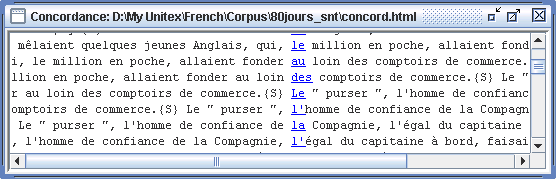
\includegraphics[width=14cm]{resources/img/fig7-locatetfst2.png}
\caption{Une concordance surprenante pour le motif
\texttt{<le.DET>}\label{fig7-locatetfst2}}
\end{center}
\end{figure}

\item \verb+<TOKEN>+\index{\verbc{<TOKEN>}} ne reconnaît pas les tokens tel que définis dans
	 \verb+tokens.txt+\index{\verbc{tokens.txt}}. Il reconnaît n'importe quelle étiquette de 
	l'automate du texte. Les étiquettes reconnues peuvent être  plus longues que les tokens si
	ce sont des étiquettes de mots composés, ou même plus courtes, si l'automate comporte une
	analyse mophologique comme \verb+un+ comme le montre la figure \ref{morphoB}, page
	\pageref{morphoB}.

\item même sans entrer dans le mode morphologique, on peut définir des variables de dictionnaire
(cf. section~\ref{dictionary-variables}). Ensuite, on peut extraire de ces variables la forme fléchie, la
forme canonique et les codes des entrées lexicales correspondantes, leur catégorie grammaticale,
leurs codes sémantiques, leurs codes flexionnels et la valeur
 \verb+zzz+ de l'attribut \verb+yyy+ s'il y figure un code de la forme \verb+yyy=zzz+.
\end{itemize}


\section{Affichage de la Table}
\label{section-table-display}
Les automates de phrases peuvent être affichées sous forme de tableau. Pour ce faire, il vous suffit
de sélectionner l'onglet "Tableau" dans la zone automate de texte. Vous verrez alors un tableau comme indiqué sur la figure \ref{fig7-table1}.


\begin{figure}[!ht]
\begin{center}
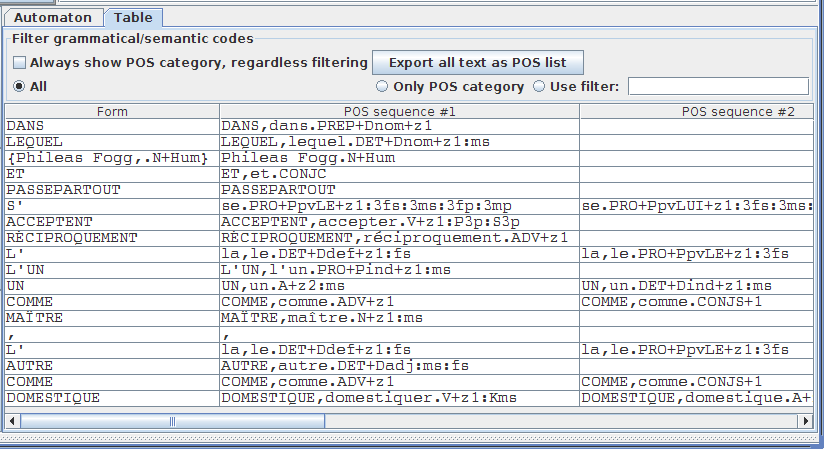
\includegraphics[width=14.5cm]{resources/img/fig7-table1.png}
\caption{Affichage d'un tableau\label{fig7-table1}}
\end{center}
\end{figure}

\bigskip
\noindent Ce tableau n'est pas tout à fait équivalent à l'automate de phrase, car il affiche
seulement les POS possibles pour chaque mot simple ou composé. Il devrait être considéré comme une
vue approximative et compacte des informations contenues dans l'automate. Vous pouvez également
filtrer les codes grammaticaux / sémantiques à afficher. Choisissez "All" et vous verrez tous les
codes. Choisissez "Only POS category" les premiers codes (supposés représenter la catégorie de la
	POS) seront affichés. Si vous choisissez "Use filter" et écrivez une expression régulière $X$,
les codes non reconnus par $X$ seront supprimés. Toute expression rationnelle POSIX est acceptée en
tant que filtre.
Vérifiez  "Always show POS category", and as said, the POS category will be kept even if not matched by the filter, if any. For instance, Figure \ref{fig7-table2} shows a filtering result, obtained with the filter \verb+^[A-Z]+ that matches any code starting with an uppercase letter, thus discarding codes like \verb+z1+.

\begin{figure}[!ht]
\begin{center}
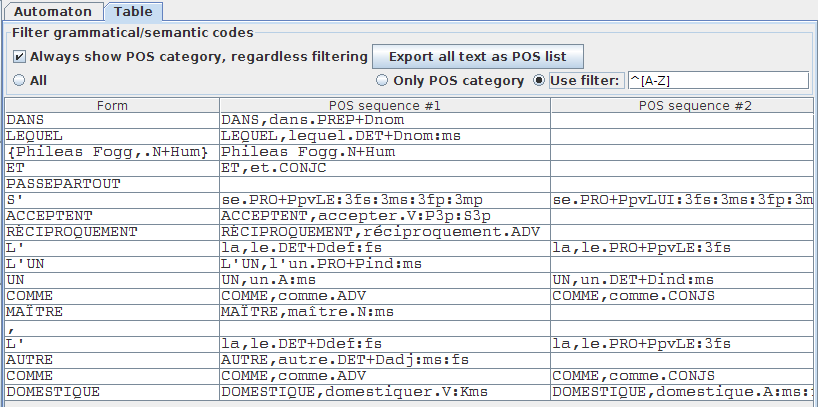
\includegraphics[width=14.5cm]{resources/img/fig7-table2.png}
\caption{Affichage d'une table filtrée\label{fig7-table2}}
\end{center}
\end{figure}
      
\bigskip
\noindent Le bouton "Export all text as POS list" peut être utilisé pour exporter ce tableau d'affichage de l'ensemble du texte automate dans un fichier texte, en utilisant un format particulier. Actuellement, cette fonctionnalité est expérimentale et peut être modifiée dans le futur. Voici un exemple de sortie:

\begin{verbatim}
(Je/N:ms:mp)|(Je/PRO/PpvIL:1fs:1ms) (suis/V:P1s)|(suis/V:Y2s:P2s:P1s) 
M/N:mp:ms . Mdiba (de/DET/Dind:fp:mp:fs:ms)|(de/PREP)|(de/PREP/z1
+de la/DET/Dind/z1:fs)|(de/PREP/z1+des/DET/Dind/z1:mp:fp)|(de/PREP/z1
+du/DET/Dind/z1:ms)|(de la/DET/Dind/z1:fs)|(des/DET/Dind/z1:mp:fp)|
(du/DET/Dind/z1:ms) LG - ville/N:fs . {S}
\end{verbatim}



\section{Le cas particulier du coréen}
\label{section-korean}
Le coréen est une langue  agglutinante qui possède une morphologie très particulière: les mots sont
formés de caractères représentant des syllabes appelés Hangul, mais un caractère Hangul correspond à
plusieurs caractères de l'alphabet JAMO. Par exemple, vous pouvez voir figure \ref{fig7-korean1} deux exemples de caractères Hangul suivis de leus équivalents en alphabet Jamo.

\begin{figure}[!ht]
\begin{center}

\includegraphics[width=4.5cm]{resources/img/fig7-korean1.png}
\caption{Caractères et leurs équivalents en alphabet Jamo
\label{fig7-korean1}}
\end{center}
\end{figure}

\noindent En outre, les morphèmes ne  correspondent pas nécéssairement à des caractères Hangul.
Par exemple, la figure \ref{fig7-korean2} montre qu'un token donné (en vert) doit être analysé
comme une combinaison de deux éléments: un verbe et un modifieur.

Le problème est que le modifieur n'est formé que d'un caractère Jamo qui se
combine avec le dernier caractère Hangul du verbe pour donner le dernier caractère
Hangul du mot entier (en vert). Les tokens en vert correspondent à des tokens non étiquetés.
Les tokens non étiquetés ne sont pas surlignés en vert pour les autres langues.

\begin{figure}[!ht]
\begin{center}
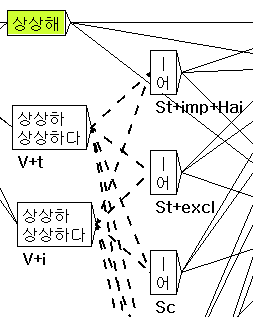
\includegraphics[width=6cm]{resources/img/fig7-korean2.png}
\caption{Décomposition d'un caractère Hangul\label{fig7-korean2}}
\end{center}
\end{figure}

\bigskip
\noindent Par conséquent, il est préférable pour les utilisateurs coréens d'écrire des grammaires
avec un mélange de Hangul et de caractères Jamo. Ainsi, une grammaire comme celle de la figure
\ref{fig7-korean3} reconnaîtra des séquences comme celles de la figure \ref{fig7-korean4}.

\begin{figure}[!ht]
\begin{center}
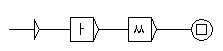
\includegraphics[width=5.5cm]{resources/img/fig7-korean3.png}
\caption{Une grammaire avec deux lettres Jamo\label{fig7-korean3}}
\end{center}
\end{figure}

\begin{figure}[!ht]
\begin{center}
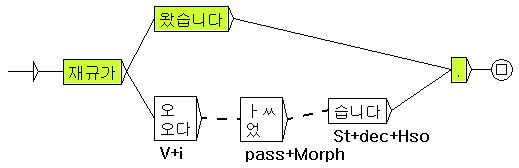
\includegraphics[width=13cm]{resources/img/fig7-korean4.png}
\caption{Automate de phrase reconnue par la grammaire de la
figure \ref{fig7-korean3}\label{fig7-korean4}}
\end{center}
\end{figure}

\bigskip
\noindent REMARQUES: 
\begin{enumerate}
\item Les lettres Jamo ne sont pas dans le fichier contenant l'alphabet coréen
	(\verb+Alphabet.txt+). NE LES AJOUTEZ PAS A CE FICHIER, parce que cela occasionnerait
    	    des disfonctionnements des programmes.\index{Alphabet!coréen}
    
\item Ce fichier alphabet contient les équivalences entre certains caractères chinois
	et certains Hangul. Dans la pratique, si la grammaire contient un caractère chinois
	qui possède un tel Hangul comme équivalent, il reconnaît celui-ci dans l'automate du texte.
	Par exemple la grammaire de la figure \ref{fig7-korean5} reconnaît la phrase de la figure
	\ref{fig7-korean4}, parce que l'alphabet contient un équivalent pour ce 
	caractère, comme le montre la figure \ref{fig7-korean6}.\index{Caractères chinois}
\end{enumerate}

\begin{figure}[!ht]
\begin{center}
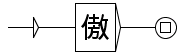
\includegraphics[width=5cm]{resources/img/fig7-korean5.png}
\caption{Une grammaire avec un caractères chinois\label{fig7-korean5}}
\end{center}
\end{figure}

\begin{figure}[!ht]
\begin{center}
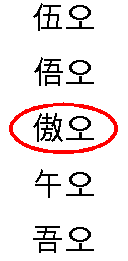
\includegraphics[width=3.5cm]{resources/img/fig7-korean6.png}
\caption{Extrait du fichier contenant l'alphabet coréen\label{fig7-korean6}}
\end{center}
\end{figure}
